
\chapter{Abtastung und Quantisierung}

\section{Analog-digital Umsetzung}

Die Verarbeitung wert- und zeitkontinuierlicher (,,analoger'') Signale mit einem digitalen Prozessor erfordert die Umsetzung des Signals in eine Zahlenfolge. Nach der numerischen Verarbeitung im Prozessor wird aus der resultierenden Zahlenfolge wieder ein analoges Signal rekonstruiert.

\begin{center}
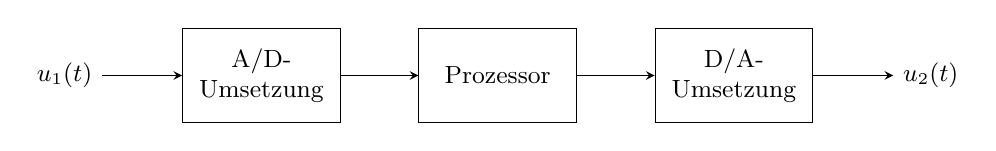
\begin{tikzpicture}[>=stealth, font=\small]
  \node at (0,0) (in) {$u_1(t)$};
  \node[draw, rectangle, minimum width=2cm, minimum height=1.2cm, align=center] at (2.5,0) (ad) {A/D-\\Umsetzung};
  \node[draw, rectangle, minimum width=2cm, minimum height=1.2cm, align=center] at (5.5,0) (proc) {Prozessor};
  \node[draw, rectangle, minimum width=2cm, minimum height=1.2cm, align=center] at (8.5,0) (da) {D/A-\\Umsetzung};
  \node at (11,0) (out) {$u_2(t)$};
  \draw[->] (in) -- (ad);
  \draw[->] (ad) -- (proc);
  \draw[->] (proc) -- (da);
  \draw[->] (da) -- (out);
\end{tikzpicture}
\end{center}

Die A/D-Umsetzung beinhaltet drei wesentliche Schritte:
\begin{enumerate}[label=\alph*.]
  \item Abtastung des zeitkontinuierlichen Signals ($\to$ Abtastwerte)
  \item Quantisierung der abgetasteten Signalwerte ($\to$ quantisierte Abtastwerte)
  \item Umsetzung der quantisierten Werte in einen digitalen Code ($\to$ Binärcode)
\end{enumerate}

Während die Abtastung unter bestimmten Bedingungen ohne Informationsverlust realisiert werden kann, ist die Quantisierung in der Regel mit einem Informationsverlust verbunden.

\section{Abtastung}

Die Abtastung eines analogen Signals führt zu einer Entnahme von ,,Signalproben'' in regelmäßigen Intervallen. In digitalen Telefonsystemen (ISDN, GSM, etc.) werden dem analogen Sprachsignal z.\,B.\ 8000 Abtastwerte pro Sekunde entnommen. Dementsprechend kann man eine \textit{Abtastfrequenz} oder \textit{Abtastrate} $f_A$ definieren:

$$
f_A = \frac{\text{Zahl der Abtastwerte}}{\text{Zeiteinheit}}
$$

Die Abtastrate wird häufig in Hz angegeben. In der Sprach- und Audiosignalverarbeitung sind typische Abtastraten:
\begin{itemize}
  \item Telefonsprache (ISDN, GSM, UMTS) \hfill 8\,kHz, 16\,kHz
  \item Audio-CD \hfill 44{,}1\,kHz
  \item DAT-Rekorder \hfill 48\,kHz
\end{itemize}

Bei Bildern sind die Abtastpunkte häufig in Form eines regelmäßigen Gitters angeordnet.

\begin{beispiel}[Abtastung eines Sinussignals]
Das analoge Signal $x(t)$ wird in regelmäßigen Abständen $T_A$ abgetastet, woraus die diskrete Folge $x[k] = x(kT_A)$ entsteht.

% Grafik: Abb. 2.68 – Oben: kontinuierliches Sinussignal x(t); unten: abgetastete Werte x(kT_A) als Impulsfolge
\end{beispiel}

\subsection*{Rekonstruktion des analogen Signals}

Bevor wir untersuchen, unter welchen Bedingungen eine Abtastung ohne Informationsverlust erreicht wird, ist die Frage zu klären, wie das analoge Signal aus den Abtastwerten rekonstruiert werden kann. Hierzu betrachten wir die drei Varianten:

\begin{itemize}
  \item \textbf{Interpolation 0.\ Ordnung, Halteglied}\\
  Die einfachste Form der Interpolation besteht darin, den Amplitudenwert zum Abtastzeitpunkt $k$ für die Dauer eines Abtastintervalls $T_A$ zu halten:
  $$
  \tilde{x}(t) = x(kT_A), \qquad kT_A \leq t < (k+1)T_A
  $$
  Die Interpolation 0.\ Ordnung ergibt ein treppenförmiges Signal.

  \item \textbf{Interpolation 1.\ Ordnung, lineare Interpolation}\\
  Bei der Interpolation 1.\ Ordnung werden die Abtastwerte abschnittsweise mit Geraden verbunden:
  $$
  \tilde{x}(t) = \bigl(x((k+1)T_A) - x(kT_A)\bigr)\,\frac{t - kT_A}{T_A} + x(kT_A),
  $$
  wobei $kT_A \leq t < (k+1)T_A$ gelten muss. Durch Einsetzen kann man sich leicht überzeugen, dass diese Gerade die Punkte $(kT_A,\, x(kT_A))$ und $((k+1)T_A,\, x((k+1)T_A))$ beinhaltet.

  \item \textbf{(Ideale) Rekonstruktion mit si-Funktionen}\\
  Gesucht sind Funktionen $g_k(t)$, so dass die Bedingung
  $$
  x(t) = \sum_{k=-\infty}^{\infty} x[k]\, g_k(t)
  $$
  mit $x[k] = x(kT_A)$ erfüllt ist. Die Funktionen $g_k(t)$ können z.\,B.\ mit Hilfe der Fouriertransformation (Vorlesung Systemtheorie~II) oder der Lagrange-Polynome gefunden werden. Es handelt sich dabei um die si-Funktion,
  $$
  g_k(t) = \operatorname{si}\!\left(\frac{t - kT_A}{T_A}\right),
  $$
  wobei $T_A = \tfrac{1}{f_A}$ das Abtastintervall bezeichnet. Somit ergibt sich die ideale Rekonstruktion zu
  $$
  \tilde{x}(t) = \sum_{k=-\infty}^{\infty} x[k]\, \operatorname{si}\!\left(\frac{t - kT_A}{T_A}\right).
  $$
\end{itemize}

% Grafik: Abb. 2.69 – Signalrekonstruktion eines Sinussignals: Interpolation 0. Ordnung (oben) und Interpolation 1. Ordnung (unten)

\subsection*{Herleitung der idealen Rekonstruktion über Lagrange-Polynome}

Die si-Funktion entspricht einem Lagrange-Polynom zur Interpolation unendlich vieler, gleichmäßig verteilter Stützstellen/Abtastwerte. Dieses wird im Folgenden gezeigt. Gegeben sei die diskrete Folge $x[k] = x(kT_A)$, für $k = 0, 1, \ldots, N-1$ und die Basisfunktionen

$$
L_k(t) = \prod_{\substack{j=0,\, j\neq k}}^{N-1} \frac{t_j - t}{t_j - t_k}
$$

mit den Werten $t_k = k \cdot T_A$ und $t_j = j \cdot T_A$. Die Interpolation

$$
\tilde{x}(t) = \sum_{k=0}^{N-1} x(t_k) \cdot L_k(t)
$$

gilt auch für unendlich viele, gleichmäßig verteilte Abtastwerte. Wir definieren hierfür die Basisfunktionen:

$$
l_k(t) = \prod_{\substack{j=-\infty,\, j\neq k}}^{\infty} \frac{t_j - t}{t_j - t_k}
= \prod_{\substack{j=-\infty,\, j\neq k}}^{\infty} \frac{jT_A - t}{jT_A - kT_A}
$$

und substituieren mit $j = n + k$:

$$
l_k(t) = \prod_{\substack{n=-\infty,\, n\neq 0}}^{\infty} \frac{(n+k)T_A - t}{nT_A}.
$$

Wir zeigen nun, dass dies einer Reihenentwicklung der si-Funktion entspricht, denn es gilt

$$
\operatorname{si}(x) = \prod_{n=1}^{\infty} \left(1 - \frac{x^2}{n^2}\right)
$$

und also auch

$$
\operatorname{si}\!\left(\frac{t - kT_A}{T_A}\right) = \prod_{n=1}^{\infty} \left(1 - \left[\frac{t - kT_A}{nT_A}\right]^2\right).
$$

Mit Hilfe der dritten binomischen Formel erhalten wir:

$$
\operatorname{si}\!\left(\frac{t - kT_A}{T_A}\right) = \prod_{n=1}^{\infty} \left(1 - \frac{t - kT_A}{nT_A}\right)\left(1 + \frac{t - kT_A}{nT_A}\right).
$$

Durch geschickte Indexerweiterung kann der Term weiter vereinfacht werden:

$$
\operatorname{si}\!\left(\frac{t - kT_A}{T_A}\right)
= \prod_{\substack{n=-\infty,\, n\neq 0}}^{\infty} \left(1 - \frac{t - kT_A}{nT_A}\right)
= \prod_{\substack{n=-\infty,\, n\neq 0}}^{\infty} \frac{(n+k)T_A - t}{nT_A}.
$$

Somit erhalten wir

$$
\tilde{x}(t) = \sum_{k=-\infty}^{\infty} x[k] \cdot \operatorname{si}\!\left(\frac{t - kT_A}{T_A}\right) = x(t).
$$

% Grafik: Abb. 2.70 – Interpolation mit si-Funktionen: Abtastwerte, eine si-Funktion pro Abtastwert, Summe aller si-Funktionen

Die maximale Signalfrequenz $f_{\max}$ muss die Bedingung $2f_{\max} < f_A$ erfüllen. Dies wird im Folgenden am Beispiel der Sinusfunktion erklärt.

\section{Das Abtasttheorem}

Die vorangegangenen Experimente und weitergehende Untersuchungen zeigen: Bei sinusförmigen Vorgängen sind mehr als zwei Abtastwerte pro Signalperiode für die eindeutige Repräsentation des Signals durch die Abtastwerte erforderlich. Wird diese Bedingung verletzt, ergibt die ideale Rekonstruktion eine Sinusfunktion bei einer Spiegelfrequenz. Da man sich beliebige Signale aus Sinussignalen zusammensetzen kann, bestimmt die in einem Signal enthaltene maximale Frequenz die erforderliche Anzahl von Abtastwerten pro Zeiteinheit.

\begin{satz}[Abtasttheorem nach Nyquist und Shannon]
Wenn die maximale Frequenz als Grenzfrequenz $f_g$ gegeben ist, muss

$$
f_A > 2f_g
$$

gelten. Die Abtastwerte werden dann in gleichmäßigen, zeitlichen Intervallen $T_A = 1/f_A$ dem Signal entnommen und mit $x(kT_A)$, $k \in \mathbb{Z}$, bezeichnet.
\end{satz}

Für $f_A = 2f_g$ ist die Signalrekonstruktion nicht eindeutig, für $f_A < 2f_g$ tritt \textit{aliasing} auf. Die Rekonstruktion mit si-Funktionen liefert in diesem Fall ein Sinussignal bei einer tieferen Frequenz

$$
\tilde{f} = f_A - f,
$$

wobei $\tilde{f}$ die sogenannte \textit{Spiegelfrequenz} darstellt. Der oben beschriebene Effekt wird in der englischen Literatur häufig als \textit{aliasing} bezeichnet.

% Grafik: Abb. 2.71 – Interpolation mit si-Funktionen: fehlerhafte Rekonstruktion bei zu geringer Abtastrate
% Grafik: Abb. 2.72 – Interpolation mit si-Funktionen und f_A = 5/(2T): korrekte Rekonstruktion
% Grafik: Abb. 2.73 – Interpolation mit si-Funktionen und f_A ≈ 5/(4T): aliasing

\section{Quantisierung}

Im Zuge der Quantisierung wird die Amplitude $x(kT_A)$ eines Signalabtastwertes zum Zeitpunkt $t = kT_A$, $k \in \mathbb{Z}$, auf eine Menge endlicher, meist fest vorgegebener Werte, den Quantisierungsniveaus, abgebildet. Damit geht in der Regel ein Informationsverlust einher. Wird der quantisierte Wert mit $x_q(kT_A)$ bezeichnet, so kann der \textit{Quantisierungsfehler} des $k$-ten Abtastwertes mit

$$
e(kT_A) = x(kT_A) - x_q(kT_A)
$$

angegeben werden.

% Grafik: Abb. 2.74 – Quantisierung des Intervalls [0,1] auf zwei (links) und vier (rechts) Werte

\section{Die Quantisierungskennlinie}

Der Zusammenhang zwischen zu quantisierendem und quantisiertem Wert kann mittels einer \textit{Quantisierungskennlinie} beschrieben werden. Zwei gebräuchliche Typen sind die Midrise- und die Midtread-Kennlinie, wie in Abb.\ 2.75 dargestellt.

Der (gleichmäßige) Quantisierer ist durch den Aussteuerbereich $[x_{\min}, x_{\max}]$ und die Stufenhöhe $\Delta x$ gekennzeichnet. In den Beispielen in Abb.\ 2.75 gilt $x_{\min} = -1$, $x_{\max} = 1$ und $\Delta x = 0{,}25$. Die Quantisierungsniveaus werden häufig auf binäre Zahlen abgebildet. Mit $w$ binären Stellen lassen sich dann maximal $2^w$ Quantisierungsniveaus indizieren.

% Grafik: Abb. 2.75 – Quantisierungskennlinien: Midrise (links) und Midtread (rechts)

\section{Der Quantisierungsfehler und seine Leistung}

Der Betrag $|e(t)|$ des Quantisierungsfehlers ist durch die halbe Quantisierungsstufenhöhe $\Delta x / 2$ beschränkt. Bei einer großen Zahl von Quantisierungsstufen hat der Quantisierungsfehler rauschartigen Charakter.

Zur Berechnung der Quantisierungsfehlerleistung betrachten wir das speziell gewählte Eingangssignal (Rampe):

$$
x(t) = \frac{t}{T}, \qquad -T \leq t \leq T,
$$

das außerhalb des betrachteten Intervalls $[-T, T]$ periodisch fortgesetzt werden kann. Dieses Signal dient als Modell für ein gleichverteiltes Signal, in dem alle Amplituden $x(t)$ mit gleicher Häufigkeit auftreten. Mit der Substitution $u = t/T$ ergibt sich die Signalleistung $P_x$ zu:

$$
P_x = \frac{1}{2T} \int_{-T}^{T} \left(\frac{t}{T}\right)^2 \mathrm{d}t
= \frac{1}{2} \int_{-1}^{1} u^2\,\mathrm{d}u
= \int_0^1 u^2\,\mathrm{d}u
= \left[\frac{1}{3}u^3\right]_0^1 = \frac{1}{3}.
$$

Der Quantisierungsfehler $e(t) = x(t) - x_q(t)$ hat Sägezahnform mit einer Periodendauer von $T_e = \Delta x \cdot T$, wobei $x_q$ auf dem Intervall $[0, \Delta x\, T]$ mit $x_q = \frac{\Delta x}{2}$ beschrieben wird. Die Leistung des Quantisierungsfehlers ergibt sich somit zu:

\begin{align*}
P_e &= \frac{1}{\Delta x\, T} \int_0^{\Delta x\, T} \bigl(x(t) - x_q(t)\bigr)^2\,\mathrm{d}t
     = \frac{1}{\Delta x\, T} \int_0^{\Delta x\, T} \left(\frac{t}{T} - \frac{\Delta x}{2}\right)^2 \mathrm{d}t \\
    &= \frac{1}{\Delta x} \int_0^{\Delta x} \left(u^2 - \Delta x\, u + \frac{\Delta x^2}{4}\right) \mathrm{d}u
     = \frac{1}{\Delta x} \left[\frac{1}{3}u^3 - \frac{1}{2}u^2 \Delta x + \frac{\Delta x^2}{4}u\right]_0^{\Delta x} \\
    &= \frac{1}{\Delta x} \left[\frac{1}{3}\Delta x^3 - \frac{1}{2}\Delta x^3 + \frac{\Delta x^3}{4}\right]
     = \frac{\Delta x^2}{12},
\end{align*}

wobei wieder $u = t/T$ substituiert wurde.

Somit erhalten wir für dieses spezielle Signal $P_e = \dfrac{\Delta x^2}{12}$.

Durch weiterführende Rechnungen kann nun gezeigt werden, dass die Formel für die Leistung des Quantisierungsfehlers näherungsweise auch für andere als das gewählte, linear ansteigende Signal gilt. Das ist dann der Fall, wenn die Zahl der Quantisierungsstufen $2^w$ ,,hinreichend'' groß ist.

\section{Dezibel}

\begin{itemize}
  \item Die Einheit Bel zeigt an, dass es sich um eine logarithmierte Verhältnisgröße handelt. Die Definition bezieht sich auf das Verhältnis zweier Leistungen $P_2$ und $P_1$:
  $$
  P = \log_{10}\!\left(\frac{P_2}{P_1}\right) \text{ [Bel]}
    = 10\log_{10}\!\left(\frac{P_2}{P_1}\right) \text{ [Dezibel]}
    = 10\,\mathrm{lg}\!\left(\frac{P_2}{P_1}\right) \text{ [dB]}
  $$
  \item Beispiel: Die Leistung des Nutzsignals wird zur Rauschleistung ins Verhältnis gesetzt. Da das Ergebnis, der Signal-zu-Störabstand oder SNR (\textit{signal-to-noise ratio}), je nach Anzahl der Quantisierungsstufen über mehrere Größenordnungen variieren kann, ist es üblich, die Verhältnisgröße zu logarithmieren.
\end{itemize}

\subsection*{Einige dB-Werte}

\begin{center}
\begin{tabular}{cc|cc}
\toprule
\multicolumn{2}{c|}{\textbf{Leistungen}} & \multicolumn{2}{c}{\textbf{Amplituden}} \\
$\dfrac{P_2}{P_1}$ & $10\,\mathrm{lg}\!\left(\dfrac{P_2}{P_1}\right)$/dB
& $\dfrac{A_2}{A_1}$ & $20\,\mathrm{lg}\!\left(\dfrac{A_2}{A_1}\right)$/dB \\
\midrule
0{,}01      & $-20$ & 0{,}01      & $-40$ \\
0{,}1       & $-10$ & 0{,}1       & $-20$ \\
0{,}25      & $-6$  & 0{,}25      & $-12$ \\
0{,}5       & $-3$  & 0{,}5       & $-6$  \\
$1/\sqrt{2}$& $-1{,}5$ & $1/\sqrt{2}$ & $-3$ \\
1           & $0$   & 1           & $0$   \\
$\sqrt{2}$  & $1{,}5$  & $\sqrt{2}$   & $3$  \\
2           & $3$   & 2           & $6$   \\
4           & $6$   & 4           & $12$  \\
10          & $10$  & 10          & $20$  \\
100         & $20$  & 100         & $40$  \\
\bottomrule
\end{tabular}
\end{center}

\subsection*{Quantisierung eines Bildsignals}

$\Rightarrow$ Die Qualität des rekonstruierten Signals hängt wesentlich von der Zahl der Quantisierungsniveaus ab.

% Grafik: Abb. 2.76 – Quantisierungsfehler e(t) = x(t) - x_q(t): Rampensignal, Sägezahnfehler, Fehlerleistung

\section{Codierung: Natürliche binäre Zahlen}

\begin{center}
\begin{tabular}{lcc}
\toprule
\textbf{Menge} & \textbf{Dezimale Zahl} & \textbf{Natürliche binäre Zahl} \\
\midrule
       & 0 & 0    \\
$\bullet$     & 1 & 1    \\
$\bullet\bullet$    & 2 & 10   \\
$\bullet\bullet\bullet$   & 3 & 11   \\
$\bullet\bullet\bullet\bullet$  & 4 & 100  \\
$\bullet\bullet\bullet\bullet\bullet$ & 5 & 101  \\
$\bullet\bullet\bullet\bullet\bullet\bullet$ & 6 & 110  \\
$\bullet\bullet\bullet\bullet\bullet\bullet\bullet$ & 7 & 111  \\
$\bullet\bullet\bullet\bullet\bullet\bullet\bullet\bullet$ & 8 & 1000 \\
\bottomrule
\end{tabular}
\end{center}

\section{Prinzip der Codierung}

Die Quantisierungsniveaus eines Quantisierers lassen sich durch einen binären Code mit endlich vielen Stellen repräsentieren.

Bei binärer Codierung ergibt sich aus der Wortbreite $w$ die Zahl darstellbarer Quantisierungsstufen zu $2^w$.

\subsection*{Typische Wortbreiten}

\begin{center}
\begin{tabular}{lcc}
\toprule
\textbf{Signal} & \textbf{Wortbreite $w$} & \textbf{Anzahl der Quantisierungsniveaus} \\
\midrule
Sprache & 8--16 Bit      & 256 -- 65\,536         \\
Audio   & 16--24 Bit     & 65\,536 -- 16\,777\,216 \\
Video   & $3 \times 8$ Bit & $3 \times 256$         \\
\bottomrule
\end{tabular}
\end{center}

\section*{Zusammenfassung}

\begin{itemize}
  \item Informationstragende Signale entstehen auf vielfältige Weise. Es werden analoge, zeitdiskrete, wertdiskrete und digitale Signale unterschieden.
  \item Sie lassen sich häufig als Summe elementarer Signale darstellen.
  \item Die digitale Verarbeitung analoger Signale erfordert eine Abtastung, Quantisierung und Codierung.
  \item Die Abtastung ist verlustfrei, wenn das Abtasttheorem eingehalten wird: $f_A > 2f_g$.
  \item Die Quantisierung führt in der Regel zu einem Informationsverlust. Die Quantisierungsfehlerleistung beträgt näherungsweise $P_e = \Delta x^2 / 12$.
\end{itemize}
